\begin{frame}
\frametitle{Organisation pratique}

\only<1>{
\begin{block}{Git et github}
	\begin{multicols}{2}
	\begin{itemize}
	\item versions
	\item système « d'issues » de Github
	\item nombreux graphiques pour visualiser l'avancement du travail
	\end{itemize}
	\begin{figure}[H]
	\begin{center}
  		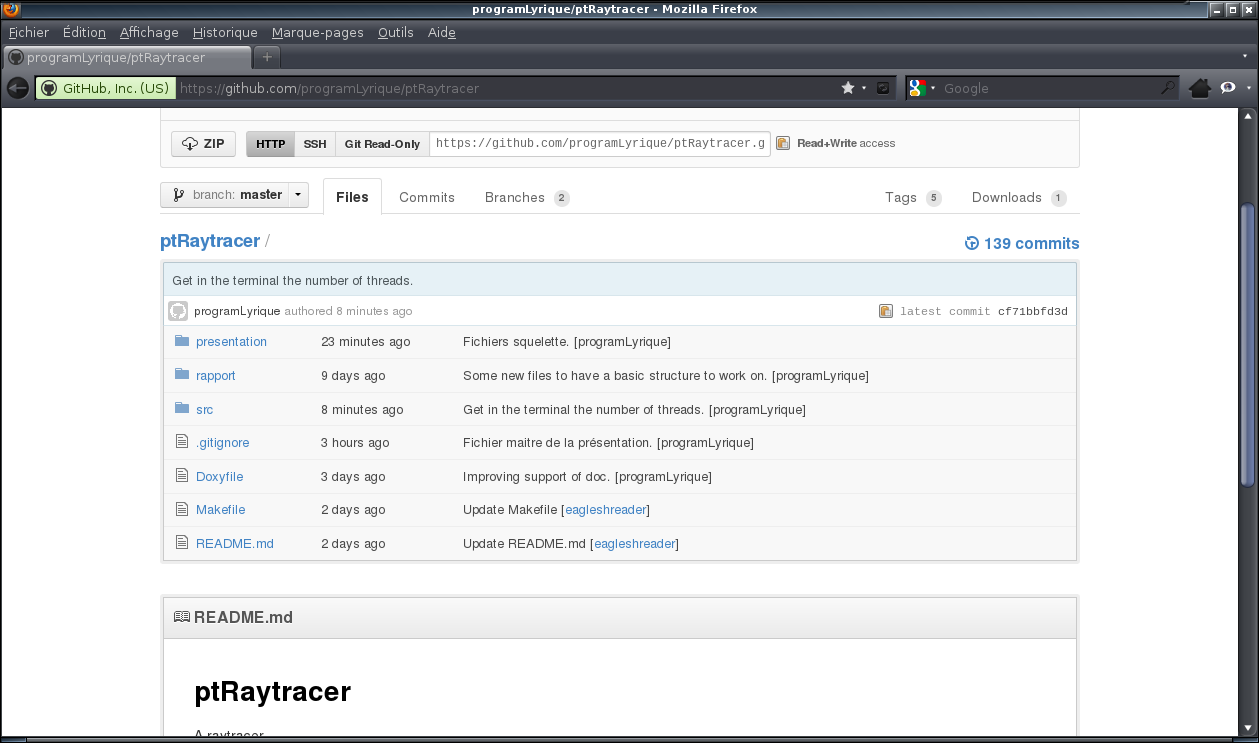
\includegraphics[scale=0.15]{Github.png}		
	\end{center}
	\caption{Page d'accueil du projet.} \label{Github}
	\end{figure}

  	\end{multicols}
\end{block}
}

\uncover<2->{
  \begin{block}{Branches}
  \only<2>{
  	\begin{figure}
  	\begin{center}
  		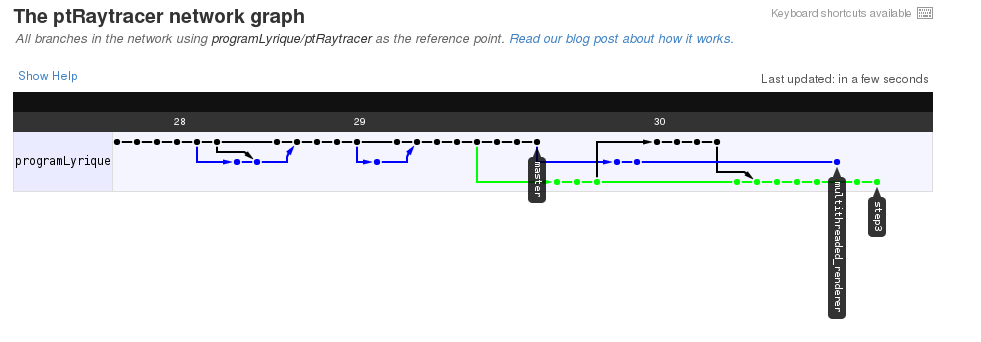
\includegraphics[scale=0.3]{arbreBranchesGit.png} 	
  	\end{center}
  	\caption{Les branches se séparent.} \label{Separent}
  	\end{figure}
	}
	\uncover<3>{	
	\begin{figure}
	\begin{center}
		  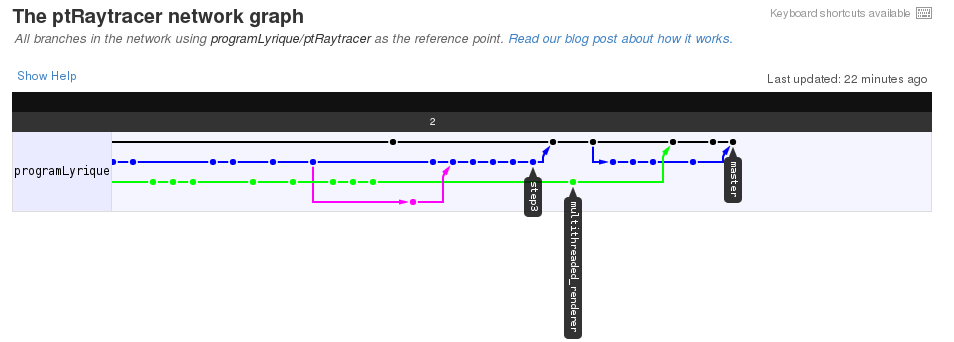
\includegraphics[scale=0.3]{arbreBranchesGit3.png}
	\end{center}
	\caption{Et se rejoignent.} \label{Rejoindre}
	\end{figure}
	}
  \end{block}
}
\end{frame}

\begin{frame}
\frametitle{Hiérarchie de classes}

\begin{center}
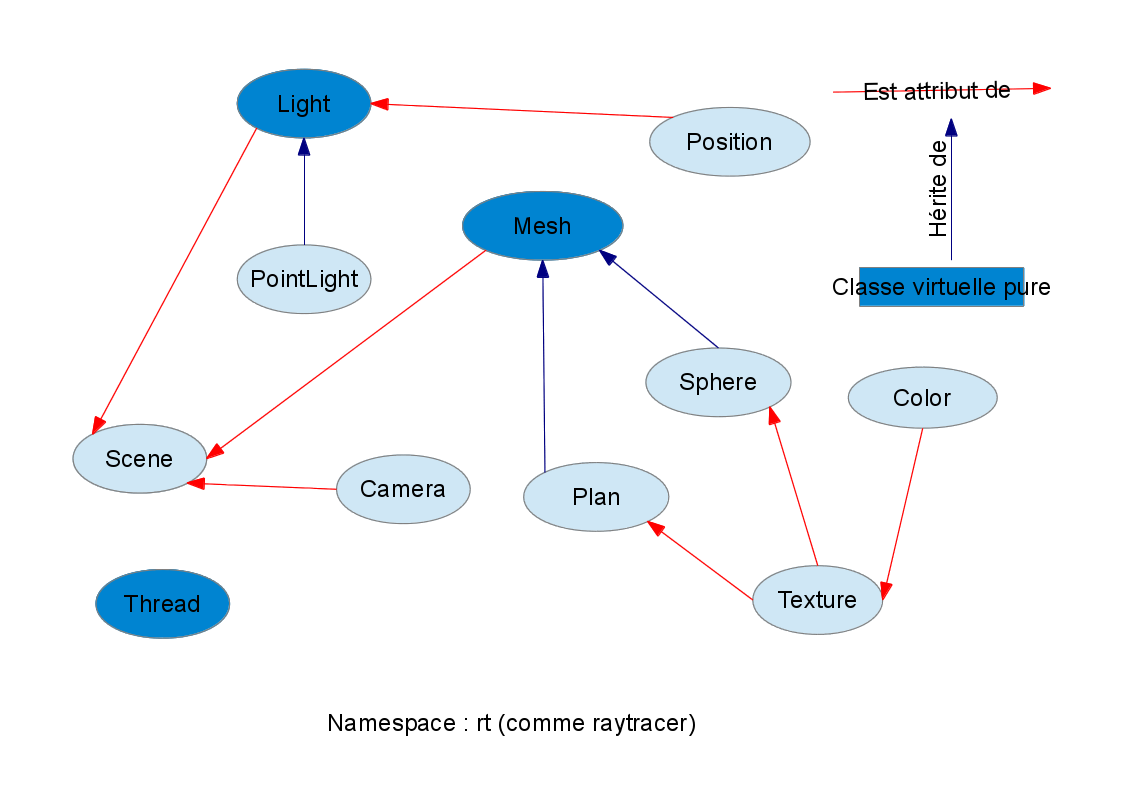
\includegraphics[scale=0.3]{hierarchie.png}
\end{center}

\begin{tikzpicture}



\end{tikzpicture}

\end{frame}